\documentclass[12pt,a4paper]{article}
\usepackage[spanish,es-tabla]{babel}

\usepackage[utf8]{inputenc} % Escribir con acentos, ~n...
\usepackage{eurosym} % s´ımbolo del euro
\newcommand{\horrule}[1]{\rule{\linewidth}{#1}} % Create horizontal rule command with 1 argument of height
\usepackage{listings}             % Incluye el paquete listing
\usepackage[cache=false]{minted}
\usepackage{graphics,graphicx, float} %para incluir imágenes y colocarlas
\usepackage{hyperref}
\hypersetup{
	colorlinks,
	citecolor=black,
	filecolor=black,
	linkcolor=black,
	urlcolor=black
}
\usepackage{multirow}
\usepackage{array}
\usepackage{diagbox}
\usepackage{listings}

\lstset{language=Java,
	keywordstyle=\color{RoyalBlue},
	basicstyle=\scriptsize\ttfamily,
	commentstyle=\ttfamily\itshape\color{gray},
	stringstyle=\ttfamily,
	showstringspaces=false,
	breaklines=true,
	frameround=ffff,
	frame=single,
	rulecolor=\color{black}}
\title{
\normalfont \normalsize 
\textsc{{\bf Técnicas de los Sistemas Inteligentes (2018-2019)} \\ Grado en Ingeniería Informática \\ Universidad de Granada} \\ [25pt] % Your university, school and/or department name(s)
\horrule{0.5pt} \\[0.4cm] % Thin top horizontal rule
\huge Práctica 2 \\ % The assignment title
\horrule{2pt} \\[0.5cm] % Thick bottom horizontal rule

\includegraphics{images/logo.png}	
}

\author{Antonio Jesús Heredia Castillo} % Nombre y apellidos

\date{\normalsize\today} % Incluye la fecha actual

%----------------------------------------------------------------------------------------
% DOCUMENTO
%----------------------------------------------------------------------------------------

\begin{document}

\maketitle % Muestra el Título
\newpage %inserta un salto de página
\tableofcontents % para generar el índice de contenidos
\listoffigures
\newpage
\section{El mapa}
El mapa que he usado para todos es el siguiente. Creo que con este mapa se puede cubrir todas los posibles casos que se den.
\begin{figure}[H]
	\centering
	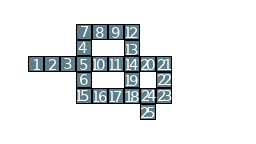
\includegraphics{images/mapa}
	\caption{}
	\label{fig:mapa}
\end{figure}
Los personajes en este mapa se encuentran en:\\
\begin{tabular}{|c|c|}
	\hline 
	Personaje & Zona \\ 
	\hline 
	bruja1 & 1 \\ 
	\hline 
	profesor1 & 25 \\ 
	\hline 
	principe1 & 14 \\ 
	\hline 
	princesa1 & 21 \\ 
	\hline 
	leonardo & 5 \\ 
	\hline 
	jugador & 13 \\ 
	\hline 
\end{tabular}\\
Los objetos se encuentran en las siguientes zonas: \\
\begin{tabular}{|c|c|}
	\hline 
	\rule[-1ex]{0pt}{2.5ex} Objeto & Zona \\ 
	\hline 
	\rule[-1ex]{0pt}{2.5ex} oro1 & 22 \\ 
	\hline 
	\rule[-1ex]{0pt}{2.5ex} oscar1 & 19 \\ 
	\hline 
	\rule[-1ex]{0pt}{2.5ex} algoritmo1 & 15 \\ 
	\hline 
	\rule[-1ex]{0pt}{2.5ex} manzana1 & 24 \\ 
	\hline 
	\rule[-1ex]{0pt}{2.5ex} rosa1 & 9 \\ 
	\hline 
\end{tabular} 
\section{Ejercicio 1}
\subsection{Tipos}
Tenemos definida la siguiente lista de tipos:
\begin{figure}[H]
	\centering
	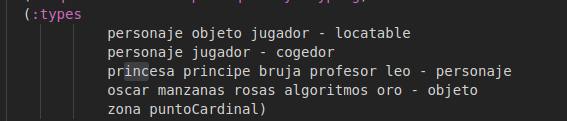
\includegraphics{images/eje1Tipos}
	\caption{}
	\label{fig:eje1tipos}
\end{figure}
He creado un tipo llamado ``locatable'', que incluirá todos los tipos que pueden estar ubicados en una posición, como son los personajes, los objetos y el jugador. Los objetos del tipo ``cogedor'' serán los que puedan tener objetos cogidos, aunque esto cambiara en los siguientes ejercicios en un principio lo diseñe así. Luego los tipos ``personaje'' y ``objeto'' que son los que pedían en el ejercicio. Cambien tengo ``zona'' que se usara para identificar las diferentes zonas del mapa y ``puntoCardinal'' para saber en que posición se encuentra una zona o la orientación del jugador. . 
\subsection{Predicados}
Los predicados que tengo son los siguientes:
\begin{itemize}
	\item zonaVecina ?zona - zona ?vecino - zona ?puntoCar - puntoCardinal : sirve para saber donde se encuentra una zona respecto a la otra. Por ejemplo zonavecina z1 z2 N, quiere decir que z2 se encuentra al norte de z1 y están conectados. 
	\item orientacionJug ?j - jugador ?orienta - puntoCardinal: indica hacia que punto cardinal se encuentra mirando un jugador.
	\item enZona ?obj - locatable ?zone - zona: indica que objeto/personaje/jugador se encuentra posicionado en una zona. 
	\item tieneObjeto ?obj - objeto ?j - cogedor: indica que objeto tiene cogido un ``cogedor''
	\item tienenUnObjeto ?j - jugador: si un jugador tiene un objeto.
	 
\end{itemize}
\subsection{Acciones}
\subsubsection{Giro a derecha}
Para el giro a la derecha solo necesito dos cosas, una que el jugador se encuentre en una zona y saber la orientación actual del jugador. Sabiendo esto simplemente, si esta por ejemplo mirando al Norte, el jugador perderá su orientación anterior y su nueva orientación sera Este. Como los giros a derecha e izquierda son diferentes vi que seria mejor tener dos acciones diferentes. 
\begin{lstlisting}
(:action GIROr-JUGADOR
	:parameters (?j - jugador ?z - zona ?o - puntoCardinal)
	:precondition (and (enZona ?j  ?z)(orientacionJug ?j ?o))
	:effect(and  
	(not(orientacionJug ?j ?o))
	(when (= ?o N)
		(orientacionJug ?j E)
	)
	(when (= ?o S)
		(orientacionJug ?j O)
	)
	(when (= ?o E)
		(orientacionJug ?j S)
	)
	(when (= ?o O)
		(orientacionJug ?j N)
	)    
	)
)
\end{lstlisting}
\subsubsection{Giro a izquierda}
Exactamente igual que el giro a la derecha. Solo que ahora el calculo de la nueva orientación cambia. Si estas mirando al norte y giras a la izquierda, la nueva posición del jugador sera Oeste.
\begin{lstlisting}
(:action GIROl-JUGADOR
	:parameters (?j - jugador ?z - zona ?o - puntoCardinal)
	:precondition (and (enZona ?j  ?z)(orientacionJug ?j ?o))
	:effect(and  
		(not(orientacionJug ?j ?o))
		(when (= ?o N)
			(orientacionJug ?j O)
		)
		(when (= ?o S)
			(orientacionJug ?j E)
		)
		(when (= ?o E)
			(orientacionJug ?j N)
		)
		(when (= ?o O)
			(orientacionJug ?j S)
		)    
	)
)
\end{lstlisting}
\subsubsection{Ir a una zona}
Esta acción es muy sencilla. Lo único que realiza es teniendo en cuenta, que la zona a la que queremos ir se encuentra en el mismo punto cardinal respecto a la zona en la que estamos que el punto cardinal al que esta orientado el jugador. Eso es lo que tenemos en las precondiciones. Como efecto el jugador deja de estar en la zona en que esta y pasa a ir a la zona que quería. 
\begin{lstlisting}
(:action IR-ZONA
	:parameters (?j - jugador ?z - zona ?z2 - zona ?o - puntoCardinal)
	:precondition (and (enZona ?j  ?z)(orientacionJug ?j ?o)(zonaVecina ?z ?z2 ?o))
	:effect(and 
		(not(enZona ?j ?z))
		(enZona ?j ?z2)
	)
)
\end{lstlisting}
La acción de coger objeto tiene como condición que el objeto y el jugador se encuentre en la misma zona y ademas que el jugador no tenga ya un objeto en la mano. El efecto es que el objeto no se encuentra en la zona y pasa a estar en el jugador.
\subsubsection{Coger objeto}
\begin{lstlisting}
(:action COGER-OBJETO
	:parameters (?j - jugador ?z - zona ?o - objeto)
	:precondition (and (enZona ?j  ?z)(enZona ?o ?z)(not(tienenUnObjeto ?j)))
	:effect(and 
		(not(enZona ?o ?z))
		(tieneObjeto ?o ?j)
		(tienenUnObjeto ?j)
	)
)

\end{lstlisting}
\subsubsection{Dejar objeto}
Para esta acción debe encontrarse en una zona el jugador y tener un objeto. El efecto sera que el jugador no tiene ya el objeto y pasa a estar en la zona. 
\begin{lstlisting}
(:action DEJAR-OBJETO
	:parameters (?j - jugador ?z - zona ?o - objeto)
	:precondition (and (enZona ?j  ?z)(tieneObjeto ?o ?j)(tienenUnObjeto ?j))
	:effect(and 
		(not(tieneObjeto ?o ?j))
		(not(tienenUnObjeto ?j))
		(enZona ?o ?z)
	)
)
\end{lstlisting}
\subsection{Dar objeto}
Aqui el jugador se debe encontrar en la misma zona que un personaje, ademas de que el jugador tenga un objeto. El efecto sera que el jugador ya no tiene el objeto y ahora lo tiene el personaje. 
\begin{lstlisting}
(:action ENTREGAR-OBJETO
	:parameters (?j - jugador ?z - zona ?o - objeto ?p - personaje)
	:precondition (and (enZona ?p  ?z)(enZona ?j  ?z)(tieneObjeto ?o ?j)(tienenUnObjeto ?j))
	:effect(and 
		(not(tieneObjeto ?o ?j))
		(tieneObjeto ?o ?p)
		(not(tienenUnObjeto ?j))
	)
)
\end{lstlisting}
\subsection{Explicación de las decisiones}
He intentado crear el mínimo posible de acciones. Pero a costa de tener posiblemente mas predicados o tipos. He intentado generalizar al maximo los tipos para que predicados como el de ``tieneObjeto'' me valga tanto para un personaje como para el jugador.
\subsection{Problema}
En el fichero de problema, tendremos como objetos todas las zonas del mapa, los personajes que vamos a colocar, los objetos a repartir y los 4 puntos cardinales. \\
En la parte de inicialización, estarán todas las zonas conectadas con sus zonas vecinas. Ademas de en que zona se encuentra los personajes, los objetos y el propio jugador.\\
Estos dos puntos nos los genera completos el parser creado en python. Que recibe como entrada lo especificado en el ejercicio y da como salida el fichero de problema para pddl. \\
Lo unico que hay que añadir al fichero generado por el parser es el ``goal'' que queremos. Que en este caso va a ser dar un objeto especifico a cada jugador. Lo de un objeto especifico para cada jugador esta hecho asi para que cuando en el ejercicio dos tengamos que optimizar no tarde demasiado.  
\section{Ejercicio 2}
\subsection{Tipos}
Los tipos son exactamente los mismo que en el ejercicio anterior, no han cambiado en nada.
\subsection{Predicados}
Los predicados también son iguales. No  he necesidad cambiarlos.
\subsection{Funciones}
Este apartado lo he tenido que añadir nuevo. ya que son necesarios para realizar la minimizacion del coste en distancia recorrida.
\begin{lstlisting}
(:functions
	(distancia ?x ?y - zona)
	(distanciaTotal)
)
\end{lstlisting}
La función ``distancia ?x ?y - zona'' nos servirá para saber cuanta distancia hay de una zona a otra con la que tiene conexión. \\
En ''distanciaTotal'' tendremos la distancia total recorrida por el jugador. Esta es la que nos servirá para minimizar.
\subsection{Accioens}
En esta ocasión hago uso de todas la acciones anteriormente descritas. Solo que añado una modificación a la accion de ir a una zona.
\subsubsection{Ir a una zona}
El único cambio que realizo en esta acción es añadir el ``increase'' que incrementara la distancia total recorrida por el jugador en la cantidad definida en ``distancia zona1 zona2''. Al haber añadido esa nueva función nos facilita mucho el cambio que había que realizar en este ejercicio. 
\begin{lstlisting}
(:action IR-ZONA
	:parameters (?j - jugador ?z - zona ?z2 - zona ?o - puntoCardinal)
	:precondition (and (enZona ?j  ?z) (orientacionJug ?j ?o)(zonaVecina ?z ?z2 ?o))
	:effect(and
		(increase (distanciaTotal) (distancia ?z ?z2))
		(not(enZona ?j ?z))
		(enZona ?j ?z2)
	)
)
\end{lstlisting}
\subsection{Problema}
En el fichero del problema no cambia mucho, simplemente el parser nos generara las funciones de distancia entre dos zonas y  inicializara la distancia total recorrida a 0.\\
Ademas añadimos como ``metric'' que se minimize la distanciaTotal. 

\section{Ejercicio 3}
En este ejercicio, existirán distintos tipos de zonas por las que el agente solo podra pasar con determinados objetos.
\subsection{Mapa}
El mapa sigue siendo el mismo, pero añadimos los nuevos objetos y los tipos de suelo. El color verde es el bosque, el color amarillo la arena, el color azul el agua y el color gris la piedra. Hay que tener en cuenta que hay objetos y personajes en la zona de bosque y agua. Para comprobar si se meten o no. 
\begin{figure}[H]
	\centering
	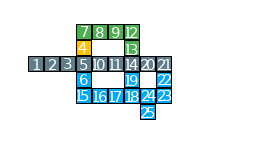
\includegraphics{images/mapaPintadoNumeros}
	\caption{}
	\label{fig:mapa}
\end{figure}
Nuevos objetos:\\
\begin{tabular}{|c|c|}
	\hline 
	Objeto & Zona \\ 
	\hline 
	bikini1 & 20 \\ 
	\hline 
	zapatillas1 & 4 \\ 
	\hline 
\end{tabular}\\\\
Los tipos de suelo son:\\
\begin{tabular}{|c|c|}
	\hline 
	Zona & Tipo \\ 
	\hline 
	1 & Piedra \\ 
	\hline 
	2 & Piedra \\ 
	\hline 
	3 & Piedra \\ 
	\hline 
	4 & Arena \\ 
	\hline 
	5 & Piedra \\ 
	\hline 
	6 & Agua \\ 
	\hline 
	7 & Bosque \\ 
	\hline 
	8 & Pricipicio \\ 
	\hline 
	9 & Bosque \\ 
	\hline 
	10 & Piedra \\ 
	\hline 
	11 & Piedra \\ 
	\hline 
	12 & Bosque \\ 
	\hline 
	13 & Bosque \\ 
	\hline 
	14 & Piedra \\ 
	\hline 
	15 & Agua \\ 
	\hline 
	16 & Agua \\ 
	\hline 
	17 & Agua \\ 
	\hline 
	18 & Agua \\ 
	\hline 
	19 & Agua \\ 
	\hline 
	20 & Piedra \\ 
	\hline 
	21 & Piedra \\ 
	\hline 
	22 & Agua \\ 
	\hline 
	23 & Agua \\ 
	\hline 
	24 & Agua \\ 
	\hline 
	25 & Agua \\ 
	\hline 
\end{tabular}\\

\subsection{Tipos}
En este ejercicio añadimos algunos tipos nuevos, que danto asi la lista de tipos:
\begin{lstlisting}
(:types  
	personaje objeto jugador - locatable
	personaje jugador - cogedor
	princesa principe bruja profesor leo - personaje
	oscar manzanas rosas algoritmos oro zapatillas bikini zapatillas bikini - objeto
	tiposSuelo zona puntoCardinal
)
\end{lstlisting}
Los nuevo tipos serán ``tipoSuelo'' que nos servira para definir los distintos tipos de suelo que tenemos en el problema.\\
Ademas añadimos los dos objetos nuevos, el bikini y las zapatillas

\subsubsection{Predicados}
Para este ejercicio he tenido que añadir algunos predicados conforme a los de ejercicios anteriores. Para realizar una reorganización en algunas acciones. 
\begin{lstlisting}
(:predicates 
	(zonaVecina ?z - zona ?vecino - zona ?puntoCar - puntoCardinal)
	(orientacionJug ?j - jugador ?orienta - puntoCardinal)
	(enZona ?obj - locatable ?zone - zona)
	(tieneObjeto ?obj - objeto ?prs - personaje)
	(manoOcupada  ?j - jugador)
	(tieneObjetoJ ?obj - objeto ?j - jugador)
	(mochilaOcupada  ?j - jugador)
	(enMochila ?obj - objeto  ?j - jugador)
	(enMano ?obj - objeto ?j - jugador)
	(tipozona ?tipe - tiposSuelo ?z - zona)

)
\end{lstlisting}
Voy a describir a continuación cuales he añadido. \\
\begin{itemize}
	\item (tipozona ?tipe - tiposSuelo ?z - zona) : nos servira para saber que tipo de suelo tiene una zona expecificamente. Es decir la zona ?z tendra sera del tipo ?tipe
	\item (enMano ?obj - objeto ?j - jugador): Nos sirve para saber que objeto tiene en la mano el jugador
	\item (enMochila ?obj - objeto  ?j - jugador): Nos sirve para saber que objeto tiene en la mochila el jugador. 
	\item (mochilaOcupada  ?j - jugador): Para saber si tiene la mochila ocupada el jugador. 
	\item (manoOcupada  ?j - jugador): Para saber si tiene la mano ocupada el jugador. 
	\item (tieneObjetoJ ?obj - objeto ?j - jugador): Este lo utilizo para acceder rapidamente si el jugador tiene un objeto en concreto, dando igual si esta en la mano en la mochila. Muy útil para usar las zapatilals y el bikini. 
\end{itemize}
\subsubsection{Funciones}
No he añadido ninguna función en este ejercicio. Aunque mantengo las anteriores en caso de que se quisiera minimizar la distancia recorrida por el jugador. 
\subsubsection{Acciones}
En este ejercicio he tenido que añadir varias acciones, aunque he intentado de minimizar la cantidad.
\subsection{Ir a una casilla sin tener objeto}
Cuando defino ir a una casilla sin tener un objeto, me refiero a sin tener un objeto de ``movilidad'' ya sea el bikini o las zapatillas. Con esta acción solo se puede mover a través de piedras y por encima de arena. 
\begin{lstlisting}
(:action IR-ZONA-SIN-OBJ
	:parameters (?j - jugador ?z - zona ?z2 - zona ?o - puntoCardinal ?t - tiposSuelo)
	:precondition (and (enZona ?j  ?z) (orientacionJug ?j ?o)(tipozona ?t ?z2 )(zonaVecina ?z ?z2 ?o))
	
	:effect(and
		(when (or (= ?t Piedra)(= ?t Arena))
			(and
				(increase (distanciaTotal) (distancia ?z ?z2))
				(not(enZona ?j ?z))
				(enZona ?j ?z2)
			)
		)
	
	)
)
\end{lstlisting}
Esto lo realizamos comprobando cual es el tipo de suelo de la zona a la que se quiere avanzar. El resultado sera el cambio de casilla.
\subsection{Ir a una casilla con zapatillas}
En esta acción nuestro jugador tendrá las zapatillas, ya sea en la mochila o en la mano, no importa. Al tener las zapatillas ademas de por las anteriores podrá ir por suelo de tipo bosque. 
\begin{lstlisting}
(:action IR-ZONA-OBJ-MOCHN-zapatillas
	:parameters (?j - jugador ?z - zona ?z2 - zona ?o - puntoCardinal ?t - tiposSuelo ?obj - zapatillas)
	:precondition (and (enZona ?j  ?z) (orientacionJug ?j ?o)(tipozona ?t ?z2 )(tieneObjetoJ ?obj  ?j )(zonaVecina ?z ?z2 ?o))
	:effect(and
	
		(when (or (= ?t Piedra)(= ?t Arena)(= ?t Bosque))
			(and
			(increase (distanciaTotal) (distancia ?z ?z2))
			(not(enZona ?j ?z))
			(enZona ?j ?z2)
		)
	)
	)
)
\end{lstlisting}
En caso de que la zona siguiente sea por una de la que se puede mover, el jugador cambiara de casilla.
\subsection{Ir a una casilla con bikni}
Como en el anterior, si el jugador tiene el bikini en su posesión, podra avanzar ademas de por la piedra y por la arena, por el agua. 
\begin{lstlisting}
(:action IR-ZONA-OBJ-MOCHN-bikini
	:parameters (?j - jugador ?z - zona ?z2 - zona ?o - puntoCardinal ?t - tiposSuelo ?obj - bikini)
	:precondition (and (enZona ?j  ?z) (orientacionJug ?j ?o)(tipozona ?t ?z2 )(tieneObjetoJ ?obj  ?j )(zonaVecina ?z ?z2 ?o))
	
	:effect(and
	
		(when (or (= ?t Piedra)(= ?t Arena)(= ?t Agua))
			(and
			(increase (distanciaTotal) (distancia ?z ?z2))
			(not(enZona ?j ?z))
			(enZona ?j ?z2)
			)
		)
	)
)
\end{lstlisting}
Si combinamos esta acción y la anterior, si el jugador tiene el bikini y las zapatillas podrá pasar tanto por el bosque como por el agua. 
\subsection{Coger/Dejar objetos}
Las siguientes acciones  de coger y dejar objetos han sufrido unos pequeños cambios. 
Para que el jugador pueda coger un objeto, este tiene que tener como precondiciñon la mano no ocupada. Esto lo especificamos con un predicado definido anteriormente. El jugador pasara a tener la mano ocupada y a tener en la mano el objeto definido y a tener el objeto de forma global.
\begin{lstlisting}
(:action COGER-OBJETO
	:parameters (?j - jugador ?z - zona ?o - objeto)
	:precondition (and (enZona ?j  ?z)(enZona ?o ?z) (not(manoOcupada  ?j)))
	:effect(and 
		(not(enZona ?o ?z))
		(enMano ?o ?j)
		(manoOcupada ?j)
		(tieneObjetoJ ?o  ?j )
	)
)
\end{lstlisting}
En el caso de dejar es parecido, solo que ahora como precondición el jugador tendra que tener el objeto necesariamente en la mano. No podrá soltarlo directamente desde la mochila. 
\begin{lstlisting}
(:action DEJAR-OBJETO
	:parameters (?j - jugador ?z - zona ?o - objeto)
	:precondition (and (enZona ?j  ?z) (manoOcupada ?j)(enMano ?o ?j))
	:effect(and 
		(not(enMano ?o ?j))
		(enZona ?o ?z)
		(not(manoOcupada ?j))
		(not(tieneObjetoJ ?o  ?j ))
	)
)
\end{lstlisting}
El jugador dejara de tener la mano ocupada, de tener el objeto en la mano y de tener el objeto de forma global. Ahora pasara ha estar el objeto en el suelo.
\subsubsection{Entregar el objeto}
A diferencia de en ejercicios anteriores, el jugador tendrá que tener el objeto necesariamente en la mano. No valdrá tenerlo en la mochila.
\begin{lstlisting}
(:action ENTREGAR-OBJETO
	:parameters (?j - jugador ?z - zona ?o - objeto ?p - personaje)
	:precondition (and (enZona ?p  ?z)(enZona ?j  ?z)(enMano ?o ?j))
	:effect(and 
		(not(enMano ?o ?j))
		(not(tieneObjetoJ ?o  ?j ))
		(tieneObjeto ?o ?p)
		(not(manoOcupada ?j))
	)
)
\end{lstlisting}
El objeto como efecto pasara a estar en posesión del personaje en cuestión y dejara de estar en la mano del jugador. 
\subsection{Guardar/Sacar objeto}
Ahora al disponer de una mochila, el jugador podra guardar y sacar objetos de ella. Para guardar un objeto, debera tener la mochila vacía ademas de tener un objeto en la mano.
\begin{lstlisting}
(:action GUARDAR-OBJETO
	:parameters (?j - jugador  ?o - objeto)
	:precondition (and (not(mochilaOcupada ?j))(manoOcupada  ?j) (enMano ?o ?j))
	:effect(and 
		(not (enMano ?o ?j))
		(not (manoOcupada ?j))
		(mochilaOcupada ?j)
		(enMochila ?o ?j)
	)
)
\end{lstlisting}
Como efecto el objeto pasara a la mochila y esta a estar ocupada. Ademas de liberar la mano del jugador.\\
Para sacar un objeto de la mochila la mano del jugador deberá estar vaciá y la mochila contener algún objeto.
\begin{lstlisting}
(:action SACAR-OBJETO
	:parameters (?j - jugador  ?o - objeto)
	:precondition (and (not(manoOcupada ?j))(mochilaOcupada  ?j) (enMochila ?o ?j))
	:effect(and 
	(not (enMochila ?o ?j))
	(not (mochilaOcupada ?j))
	(manoOcupada ?j)
	(enMano ?o ?j)
	)
)
\end{lstlisting}
\subsection{Problema}
En el fichero de problema no cambian ni los objetivos ni la métrica. El parser solo añadirá a los objetos los distintos tipos de suelo y también añadirá los dos nuevos objetos(bikini y zapatilla)\\
En la zona de inicialización se inicializara de que tipo de zona es cada zona. 
\section{Ejercicio 4}
En este ejercicio se añade diferentes puntuaciones a la entrega de objetos.
\subsection{Tipos}
No añado ningun tipo nuevo al dominio.
\subsection{Predicados}
No añado ningun predicado nuevo al dominio.
\subsection{Funciones}
Aquí si añado algunas funciones nuevas que paso a explicar a continuación. 
\begin{itemize}
\item (puntosMaximos): Aqui se guardara los puntos necesarios para que el ``juego'' acabe. 
\item (puntosTotales): La cantidad de puntos que tiene el jugador por ahora.
\item (puntosDa ?x - objeto ?y - personaje) : la determinada cantidad de puntos que da un objeto a un personaje.  
\end{itemize}
\subsection{Acciones}
En este ejercicio solo cambia una acción y es la de entregar objeto al personaje. Añadimos un ``increase'' que añadira a la función puntosTotales la cantidad de puntos definida por (puntosDa ?x - objeto ?y - personaje).  
\begin{lstlisting}
(:action ENTREGAR-OBJETO
	:parameters (?j - jugador ?z - zona ?o - objeto ?p - personaje)
	:precondition (and (enZona ?p  ?z)(enZona ?j  ?z)(enMano ?o ?j))
	:effect(and 
		(not(enMano ?o ?j))
		(not(tieneObjetoJ ?o  ?j ))
		(tieneObjeto ?o ?p)
		(not(manoOcupada ?j))
		(increase (puntosTotales) (puntosDa ?o ?p))
	)
)
\end{lstlisting}
Con esto conseguimos tener la función puntosTotales actualizada cada vez que se entrega un objeto.
\subsection{Problema}
Ahora en el problema cambiaremos el goal.Ahora el objetivo del jugador sera obtener al menos 50 puntos.
\begin{lstlisting}
(:goal 
	(AND 
		(>= (puntosTotales) (puntosMaximos))
	)
)
\end{lstlisting} 
Ademas el parser añadira al fichero de problema cuantos puntos dará cada objeto a cada personaje. Por ejemplo un oscar le da a la bruja 4 puntos. 
$$(= (puntosDa oscar1 bruja1) 4)$$
El parser también inicializara el valor de $$(= (puntosTotales) 0)$$ y 
$$(= (puntosMaximos) 50)$$
\section{Ejercicio 5}
En este ejercicio se limitara la cantidad de objetos que puede tener un determinado personaje. \\
En este ejercicio no añado ni predicados ni tipos nuevo, pero si funciones.
\subsection{Funcioness}
Tengo dos nuevas funciones.\\
La función $(tamanioBolsillo ?x - personaje)$ no dirá el tamaño del bolsillo de un personaje.\\
La función $(cantidadObjetos ?x - personaje)$ nos dirá la cantidad de objetos que lleva ya el personaje. \\
Estas dos funciónes nos servira para no dar mas objetos de los que tiene capacidad a un personaje. Esto lo controlaremos con las acciones. 
\subsection{Acciones}
\subsubsection{Dar objeto}
La función dar objeto es la que tiene que controlar que no demos mas objetos que los que tiene capacidad un determinado personaje. El tamaño del bolsillo mágico de cada personaje se instancia en el archivo de problema y de ahí se coge. La acción comprobara antes de dar el objeto que el personaje tiene capacidad y si tiene, se lo da, ademas incrementa en 1 la cantidad total de objetos que tiene el personaje.  
\begin{lstlisting}
(:action ENTREGAR-OBJETO
	:parameters (?j - jugador ?z - zona ?o - objeto ?p - personaje)
	:precondition (and (enZona ?p  ?z)(enZona ?j  ?z)(enMano ?o ?j))
	:effect(and 
	(when	(and (< (cantidadObjetos ?p) (tamanioBolsillo ?p)))
		(and
			(not(enMano ?o ?j))
			(not(tieneObjetoJ ?o  ?j ))
			(tieneObjeto ?o ?p)
			(not(manoOcupada ?j))
			(increase (puntosTotales) (puntosDa ?o ?p))
			(increase (cantidadObjetos ?p) 1)
		)
	)
	)
)
\end{lstlisting}
\subsection{Problema}
En el fichero de problema el parser añadirá la capacidad que tiene cada personaje ademas de inicializar a 0 la cantidad de objetos que tiene cada uno. El objetivo no cambia.
\section{Ejercicio 6}
En este ejercicio habrá varios jugadores. Y ambos tendrá que llegar a un mínimo de puntos, que este puede cambiar de uno a otro. Ademas se tendrá que llegar al objetivo de mínimo de puntos. 
\subsection{Funciones}
En este ejercicio volvemos a añadir dos funciones muy parecidas a las del ejercicio anterior. 
La función $(puntosJugador ?j - jugador)$ nos indicara cuantos puntos tiene cada jugador.\\
La función $(puntosMinimoJugador ?j - jugador)$ nos indicara cuantos puntos necesita cada jugador.\\
Con estas dos funciones podremos controlar el objetivo necesario.
\subsection{Acciones} 
\subsection{Dar objeto}
Volvemos a modificar solo la acción de dar objeto a un personaje. En esta función añadiremos un incremento en los puntos que tiene cada jugador. Los puntos se incrementan en función de la cantidad de puntos que da dar un determinado objeto a un determinado personaje ($(puntosDa ?o ?p)$).
\begin{lstlisting}
(:action ENTREGAR-OBJETO
	:parameters (?j - jugador ?z - zona ?o - objeto ?p - personaje)
	:precondition (and (enZona ?p  ?z)(enZona ?j  ?z)(enMano ?o ?j))
	:effect(and 
	(when (and (< (cantidadObjetos ?p) (tamanioBolsillo ?p)))
		(and
			(not(enMano ?o ?j))
			(not(tieneObjetoJ ?o  ?j ))
			(tieneObjeto ?o ?p)
			(not(manoOcupada ?j))
			(increase (puntosTotales) (puntosDa ?o ?p))
			(increase (cantidadObjetos ?p) 1)
			(increase (puntosJugador ?j) (puntosDa ?o ?p))
			)
		)
	)
)
\end{lstlisting}

\subsection{Problema}
El objetivo ahora ademas de tener una cantidad mínima de puntos totales necesarios también tendrá la cantidad mínima de puntos por jugador. 
\begin{lstlisting}
(:goal 
	(AND 
		(>= (puntosTotales) (puntosMaximos))
		(>= (puntosJugador player1) (puntosMinimoJugador player1))
		(>= (puntosJugador player2) (puntosMinimoJugador player2))
	)
)
\end{lstlisting}
Ademas el parser añade los puntos minimos que necesita cada jugador y inicializa a 0 los puntos que tiene hasta ahora. 
\section{Parser}
El parser esta escrito en Python. Hay un parser y un fichero sin procesar y otro procesado del problema para cada ejercicio. Aunque he intentado realizarlo lo mejor posible, es muy rigido, es decir no te puedes dejar un espacio o lineas en blanco. No obstante funciona de forma adecuada para todos los ejercicios. La parte de los objetivos no la completa ya que entiendo que es algo que puede variar mucho mas entre ejercicio.
\end{document}